\documentclass[letterpaper]{article}
\usepackage[submission]{aaai2027}
\usepackage[hyphens]{url}
\usepackage{graphicx}
\urlstyle{rm}
\def\UrlFont{\rm}
\usepackage{natbib}
\usepackage{caption}
\usepackage{amsmath}
\usepackage{amssymb}
\usepackage{algorithm}
\usepackage{algorithmic}
\usepackage{booktabs}
\frenchspacing

\pdfinfo{/TemplateVersion (2027.1)}
\setcounter{secnumdepth}{2}

\newcommand{\method}{\textsc{Veil}}
\newcommand{\tpr}{\ensuremath{\mathrm{TPR}@1\%\mathrm{FPR}}}
\newcommand{\norm}[1]{\left\lVert #1 \right\rVert_2}

\title{VEIL: Variance-Echoed Instance-Less Prompt Learning for Membership-Resistant Federated Vision--Language Models}
\author{Anonymous Submission}
\affiliations{}

\begin{document}
\maketitle

\begin{abstract}
Federated prompt learning adapts a frozen vision--language model by exchanging
only compact prompt updates, but compactness does not imply membership privacy:
confidence trajectories, update alignment, and released prompts can still
separate members from non-members.  We introduce \method{} (Variance-Echoed
Instance-Less Prompt Learning), a client-local defense
that prevents individual examples from serving as direct prompt-training
anchors.  Each client estimates class-conditional geometry in the frozen CLIP
embedding space, replaces each private feature with its class prototype, and
generates covariance-shaped ``echoes'' without transmitting features, means, or
covariances.  A clipping-and-perturbation step further smooths the
prompt delta before FedAvg aggregation, and a label-preserving temperature map
moderates confidence from the released model.  We evaluate a protocol-aware attacker
with six membership attacks at the stringent true-positive rate at 1\% false-
positive rate (\tpr{}) operating point.  Our benchmark uses label-matched
member/non-member candidates, audit-specific random generators, three image
datasets, and repeated non-IID partitions.  Averaged over datasets, \method{}
obtains the lowest six-attack mean \tpr{} among the evaluated FedAvg defenses
(0.0145), 15.3\% and 24.2\% relatively below Prompt-DP and HAMP, while matching
Prompt-DP mean accuracy within 0.12 percentage points.  It improves both privacy
summaries on Caltech101 but not on DTD, so we do not claim universal dominance.
The private-mechanism study further exposes attack-specific failures hidden by
one aggregate score.  Local distributional surrogates are thus an empirical
complement to formal privacy mechanisms, not a differential-privacy guarantee.
\end{abstract}

\section{Introduction}

Vision--language models such as CLIP provide transferable representations that
can be adapted with a small set of learned context tokens rather than full-model
fine-tuning \citep{radford2021clip,zhou2022coop}.  Federated prompt learning
combines this parameter efficiency with decentralized optimization: clients
retain their images and communicate only prompt updates
\citep{mcmahan2017fedavg,zhao2023fedprompt,guo2024promptfl}.  The resulting protocol is cheap,
but it exposes a recurring sequence of low-dimensional, task-specific updates.
Such updates and the released prompt can leak whether a candidate example was
used for local training, even when the frozen backbone never leaves the server.

Membership inference is particularly consequential at low false-positive rates,
where an attacker can make high-confidence claims about a small number of people
or records \citep{shokri2017membership,carlini2022membership}.  Existing
defenses offer incomplete choices.  Differentially private optimization gives a
formal guarantee, but noise can destabilize prompt learning in strongly non-IID,
few-shot regimes \citep{abadi2016dpsgd,duan2023privateprompt}.  Output-centered
methods such as HAMP reduce overconfidence, yet do not directly erase update
alignment \citep{chen2024hamp}.  Private federated prompt and low-rank training
mechanisms, including DP-FPL and FedASK (also called FedSAK in some project
documentation), change the communicated parameterization
but remain subject to empirical auditing \citep{dpfpl2025,fedask2025}.

We ask whether the client can preserve the class structure needed for prompt
learning without repeatedly optimizing on identifiable instance directions.
Our answer is \method{}.  Like a veil that preserves a silhouette while hiding
identity, the client presents the prompt optimizer with variance-shaped echoes
of its class distribution: the semantic outline remains recognizable, but the
individual that generated it is obscured.
The method operates entirely in the frozen image-embedding space.  It replaces
raw instance anchors with local class prototypes, samples low-rank covariance-
shaped echoes, smooths only the trainable prompt delta before upload, and
tempers final released logits without changing their predicted class.

Our contributions are fourfold:
\begin{itemize}
    \item We formulate instance-anchor exposure as a distinct membership channel
    in federated soft-prompt tuning and introduce class-geometry echo training to
    reduce that channel without sharing auxiliary client statistics.
    \item We develop \method{}, combining prototype replacement, implicit
    covariance sampling, prompt-update smoothing, and label-preserving output
    tempering while keeping CLIP frozen and aggregating only trainable parameters.
    \item We construct a strict protocol-aware audit covering FedMIA confidence,
    FedMIA update alignment, their fixed joint score, Nasr-style passive white-box
    inference, RMIA, and quantile-regression MIA.  Candidate label histograms are
    exactly matched and audit loading is isolated from the training RNG.
    \item We organize a multi-dataset evaluation into two complementary studies:
    defenses under a common FedAvg backbone, and attack behavior under DP-FPL and
    FedASK.  We report clean accuracy, per-attack \tpr{}, worst-attack \tpr{},
    and variation across seeds.
\end{itemize}

\section{Related Work}

\paragraph{Federated prompt learning.}
Prompt tuning adapts a pretrained model through a small trainable context
\citep{lester2021prompt,zhou2022coop}.  FedAvg supplies the standard weighted
aggregation rule for decentralized optimization \citep{mcmahan2017fedavg}, and
FedPrompt and PromptFL demonstrate the communication advantages of exchanging
prompts \citep{zhao2023fedprompt,guo2024promptfl}.  DP-FPL factorizes global and personalized prompts
and perturbs private updates, while FedASK aggregates both low-rank factors
through an asymmetric double-sketch mechanism
\citep{dpfpl2025,fedask2025}.  Our work does not replace these mechanisms; it
studies a complementary defense at the client representation and upload levels.

\paragraph{Membership inference and auditing.}
Black-box membership inference exploits differences in model behavior on
training and non-training examples \citep{shokri2017membership}.  Nasr et al.
extend the threat to passive and active white-box adversaries
\citep{nasr2019comprehensive}.  Modern attacks emphasize calibrated likelihood
ratios and low-FPR evaluation \citep{carlini2022membership,zarifzadeh2024rmia},
while scalable quantile regression learns input-dependent non-member thresholds
\citep{bertran2023quantile}.  FedMIA uses other clients as a per-round null
population and measures confidence or gradient--update alignment
\citep{zhu2025fedmia}.  We retain each attack's information source but specialize
features to frozen-backbone prompt tuning.

\paragraph{Membership defenses.}
DP-SGD clips per-example gradients and adds Gaussian noise
\citep{abadi2016dpsgd}; private prompt learning applies related ideas to a much
smaller parameter space \citep{duan2023privateprompt}.  HAMP combines high-
entropy soft targets, entropy regularization, and low-confidence prediction
mapping \citep{chen2024hamp}.  In contrast, \method{} intervenes before the
prompt loss sees an individual image embedding.  Its geometry sampling resembles
distributional feature augmentation, but all class statistics remain local and
the objective is membership resistance rather than data sharing or domain
generalization.

\section{Motivation: Compact Updates Still Carry Individual Traces}

Freezing CLIP eliminates backbone-gradient leakage but does not eliminate three
prompt-specific membership channels.  First, the loss and confidence trajectory
of a member can remain systematically different over rounds.  Second, the
gradient induced by a candidate can align with the observed client prompt delta.
Third, a final prompt may retain an input-dependent confidence gap.  Because the
trainable prompt is small, each private mini-batch contributes to the same compact
parameter block; parameter efficiency can therefore concentrate rather than
remove membership evidence.

A direct response is to perturb the prompt gradient.  In few-shot non-IID
training, however, individual classes may be represented by only a handful of
local examples, so indiscriminate noise can remove useful directions and cause
large seed-to-seed utility variation.  Our working hypothesis is that prompt
learning primarily needs class-level semantic position and local variation,
whereas repeatable instance-level directions form an avoidable membership
channel.  This motivates the
following design requirements: (i) no raw member feature acts as an optimization
anchor; (ii) local class variation is preserved without exporting statistics;
(iii) the upload is smoothed because representation replacement alone cannot
remove all update-side evidence; (iv) confidence from the final released model
is moderated without changing its decision; and (v) the mechanism remains
compatible with a frozen backbone and standard FedAvg.

\section{Problem Formulation and Threat Model}

There are $K$ clients.  Client $k$ owns
$D_k=\{(x_i,y_i)\}_{i=1}^{n_k}$ and the server maintains trainable prompt
$\theta^t$.  The CLIP image encoder $\phi$ and text encoder $\psi$ are frozen.
Given class $c$, $\psi(c;\theta)$ denotes its normalized text representation.
Only tensors whose \texttt{requires\_grad} flag is true are optimized and
aggregated.  Under FedAvg, the server computes
\begin{equation}
\theta^{t+1}=\sum_{k\in S_t}\frac{n_k}{\sum_{j\in S_t}n_j}\theta_k^{t+1}.
\end{equation}

The adversarial server observes protocol messages from all selected clients and
released prompt checkpoints, and can query the released model.  It does not see
raw client images, local feature banks, class means, or covariance factors.  For
a candidate $(x,y)$ and target client $k^*$, it predicts whether
$(x,y)\in D_{k^*}$.  We evaluate at \tpr{}, following low-FPR membership
auditing practice \citep{carlini2022membership}.  \method{} is an empirical
defense: its Gaussian upload perturbation is not claimed to satisfy a calibrated
$(\epsilon,\delta)$-DP bound.

\section{VEIL}

Here, ``instance-less'' qualifies the prompt-optimization anchors: clients still
use their instances locally to estimate class geometry, but no individual image
embedding is supplied directly to the prompt loss.

\subsection{Local Class Geometry}

Each client first builds a detached feature bank using the frozen image encoder:
\begin{equation}
z_i=\frac{\phi(x_i)}{\norm{\phi(x_i)}},\qquad
F_{k,c}=\{z_i:y_i=c\}.
\end{equation}
For every observed local class, it computes
\begin{equation}
\mu_{k,c}=\frac{1}{n_{k,c}}\sum_{z\in F_{k,c}}z,
\quad
Z_{k,c}=\begin{bmatrix}(z_1-\mu_{k,c})^\top\\\cdots\\
(z_{n_{k,c}}-\mu_{k,c})^\top\end{bmatrix}.
\end{equation}
No quantity in $F_{k,c}$, $\mu_{k,c}$, or $Z_{k,c}$ is transmitted.

\subsection{Prototype Replacement and Geometric Echoes}

For every label in a local batch, \method{} replaces the corresponding private
image feature by the normalized class prototype
\begin{equation}
z^{\mathrm{proto}}_{k,c}=\frac{\mu_{k,c}}{\norm{\mu_{k,c}}}.
\end{equation}
It then draws $m$ geometric echoes.  With
$e\sim\mathcal{N}(0,I_{n_{k,c}})$, define
\begin{equation}
\beta_{k,c}=\frac{e^\top Z_{k,c}}{\sqrt{n_{k,c}-1}},\qquad
\tilde z_{k,c}=\frac{\mu_{k,c}+s\beta_{k,c}}
{\norm{\mu_{k,c}+s\beta_{k,c}}}.
\label{eq:echo}
\end{equation}
Conditioned on the local bank, $\beta_{k,c}$ has the empirical class covariance
without explicitly forming or decomposing a $d\times d$ covariance matrix.  If
$n_{k,c}<2$, we use isotropic noise with standard deviation 0.02.  Anchoring at $\mu_{k,c}$ is crucial:
anchoring at $z_i$ would preserve the individual direction we seek to suppress.

\subsection{Prompt Objective}

Let $B_k^{\mathrm{echo}}$ contain one prototype and $m$ echoes for every batch
label.  Text features remain differentiable with respect to $\theta$ while all
image features are detached.  With CLIP logit scale $\tau$, client $k$ minimizes
\begin{equation}
\mathcal{L}_k(\theta)=\frac{1}{|B_k^{\mathrm{echo}}|}
\sum_{(z,y)\in B_k^{\mathrm{echo}}}
-\log\frac{\exp(\tau z^\top\psi(y;\theta))}
{\sum_{c'}\exp(\tau z^\top\psi(c';\theta))}.
\label{eq:objective}
\end{equation}
The selected operating point uses $m=3$, $s=0.6$, and no entropy penalty.

\subsection{Prompt-Delta Smoothing}

Representation replacement targets instance anchors, but an update can still
encode rare class structure.  For local prompt delta
$\Delta_k=\theta_k^{t+1}-\theta^t$, we apply
\begin{align}
\Delta_k^{\mathrm{clip}}&=\Delta_k\min\left(1,
\frac{C}{\norm{\Delta_k}}\right),\\
\bar\Delta_k&=\Delta_k^{\mathrm{clip}}+\xi_k,
\quad \xi_k\sim\mathcal{N}(0,(\rho C)^2I).
\end{align}
The client uploads $\theta^t+\bar\Delta_k$.  We use $C=0.5$ and $\rho=0.11$.
The randomness is client-, round-, and purpose-specific, and each released state
is a detached tensor copy.

\subsection{Released-Output Tempering}

The released model maps logits $\ell(x;\theta)$ to
\begin{equation}
\ell^{\mathrm{rel}}(x;\theta)=\ell(x;\theta)/T,
\qquad T=4.
\end{equation}
This deterministic map preserves the top-1 prediction and hence clean accuracy,
but reduces the scale of released confidence.  It is applied only to final-model
queries: with \texttt{calibrate\_observations=false}, the round-level confidence
and update signals remain unmodified.  We use no logit-margin cap.

\begin{algorithm}[t]
\caption{One \method{} Client Update}
\label{alg:veil}
\begin{algorithmic}[1]
\REQUIRE Frozen image encoder $\phi$, prompt $\theta^t$, local data $D_k$
\STATE Encode detached normalized features and construct $(\mu_{k,c},Z_{k,c})$
\FOR{each local mini-batch}
  \STATE Replace every image feature by its normalized class prototype
  \STATE Draw $m$ covariance-shaped echoes using Eq.~\eqref{eq:echo}
  \STATE Update only $\theta$ using Eq.~\eqref{eq:objective}
\ENDFOR
\STATE Clip $\theta_k^{t+1}-\theta^t$ to norm $C$ and add $\mathcal{N}(0,(\rho C)^2I)$
\RETURN Detached prompt state $\theta^t+\bar\Delta_k$
\end{algorithmic}
\end{algorithm}

\subsection{Privacy--Utility Interpretation and Cost}

Prototype replacement removes direct instance anchors; geometric echoes restore
class-conditioned diversity; upload smoothing targets the residual protocol
channel; and output tempering moderates the final-query channel.  These roles
target distinct information paths, but their empirical contributions need not
be equal.  In the current implementation,
the feature-bank pass costs one frozen image-encoder evaluation per local example
per round.
For embedding dimension $d$, storing the detached bank costs $O(n_kd)$ and
generating $m$ echoes costs $O(mn_bd)$ for batch size $n_b$.  No extra server
state or communication is introduced beyond the prompt update.

\section{Experimental Methodology}

\subsection{Research Questions}

We organize the study around four questions.  \textbf{RQ1:} Under a common
FedAvg backbone, how does \method{} compare with no defense, Prompt-DP, and
HAMP across attacks and datasets?  \textbf{RQ2:} Which attacks remain effective
when the training mechanism is DP-FPL or FedASK?  \textbf{RQ3:} What utility is
paid for lower worst-attack leakage?  \textbf{RQ4:} Which components of
\method{} account for the observed trade-off?

\subsection{Datasets and Federated Protocol}

We use Flowers102 \citep{nilsback2008flowers}, Caltech101
\citep{fei2004caltech}, and DTD \citep{cimpoi2014dtd}.  They respectively test
fine-grained appearance, heterogeneous objects, and material texture.  Every
dataset uses 16 labeled examples per class from its training partition, while
evaluation uses the complete held-out test partition; DTD uses its first
predefined fold.  We partition the few-shot training set over
10 clients with a Dirichlet distribution of concentration $\alpha=0.1$, select
all 10 clients per round, and train for five global rounds with one local epoch.
The batch size is 16, learning rate is $10^{-3}$, and prompt length is 16.
Standard prompt updates use SGD with zero momentum and weight decay; private
mechanisms use their method-specific update rules at the same learning rate.
The audit target is client 0.  Reported aggregates use seeds 42--44 unless stated
otherwise.  Formal runs use two NVIDIA RTX 4090 GPUs; CLIP ViT-B/32 is loaded
from local storage and remains frozen.  The host uses an Intel Core i5-14600KF,
two 24-GB RTX 4090 GPUs, Linux 6.8, Python 3.9.21, PyTorch 2.7.1 with CUDA 12.8,
Transformers 4.57.3, and NumPy 1.26.3.
The main matrix contains 54 independent runs (three datasets, three seeds, and
six mechanisms); the component study adds seven Flowers102 seed-42 runs.  Each
process occupies one GPU, and no process silently falls back to CPU.

\begin{table}[t]
\centering
\begin{tabular}{lrrrr}
\toprule
Dataset & Classes & Train & Test & Mean/client\\
\midrule
Flowers102 & 102 & 1,632 & 6,149 & 163.2\\
Caltech101 & 101 & 1,616 & 5,647 & 161.6\\
DTD & 47 & 752 & 1,880 & 75.2\\
\bottomrule
\end{tabular}
\caption{Dataset scale after the common 16-shot-per-class protocol.  The last
column is the arithmetic mean over 10 clients; actual client counts are unequal
under the $\alpha=0.1$ Dirichlet partition.  Test counts cover the complete
evaluation partitions.}
\label{tab:datasets}
\end{table}

We tune \method{} on Flowers102 seeds 42--43 and reserve seed 44 as a held-out
replication.  The development sweep covers echo counts $m\in\{0,3,6\}$,
geometry scales $s\in\{0.45,0.60\}$, class-mean versus individual anchors,
prototype/drop/noisy-prototype replacement, clipping thresholds
$C\in\{0.05,0.5\}$, and upload noise ratios
$\rho\in\{0.07,0.11,0.15,0.20\}$.  The release temperature is $T=4$ unless
ablated.  We select the point with the lowest
worst-attack \tpr{} among configurations whose mean development accuracy is at
least 0.60, breaking ties by higher accuracy.  The selected parameters are then
frozen for Caltech101 and DTD.
All split, initialization, client, and audit generators are keyed by the reported
seed.  DP mechanisms keep \texttt{reproducible\_dp\_noise=false}; their Gaussian
draws intentionally use a private non-deterministic generator, so seed labels
identify the repeated scenario rather than fixing privacy noise byte-for-byte.

\subsection{Baselines}

The FedAvg defense study includes: no defense; Prompt-DP with per-example prompt
gradient clipping at 1.0 and Gaussian noise multiplier 1.0; HAMP with true-class
soft-target mass 0.6, entropy weight 0.05, and output temperature 4; and
\method{}.  The private-training study evaluates DP-FPL with rank 4, one local
private step, local/global clipping 1.0, and noise multipliers 0.3/0.1; and
FedASK with rank/sketch size 16, ten local private steps, clipping 1.0, and noise
multiplier 1.0.  Method-specific update rules follow their respective public
implementations; all scenario and audit fields remain fixed.
Prompt-DP is applied only to trainable CLIP prompt tensors.  Because a
non-differentiable randomized HAMP release would make gradient-based auditors
undefined, we use its high-entropy training objective and a deterministic,
argmax-preserving temperature map; this is reported as a prompt-learning
adaptation rather than a byte-identical reproduction.  Likewise, DP-FPL's
global/local factors and FedASK's two-stage sketches are mapped to CLIP prompt
matrices; their original language-model tasks are not reproduced.
FedAvg, Prompt-DP, HAMP, \method{}, and FedASK release one shared prompt.  DP-FPL
retains its defining persistent client-local residual and is evaluated with each
client's own global-plus-local prompt; accuracies are then micro-averaged over
the same client test partitions.  Forcing DP-FPL to discard its local state
would no longer reproduce its stated algorithm.

\subsection{Attacks and Metrics}

We evaluate FedMIA-I (confidence), FedMIA-II (gradient--update cosine), a fixed
joint z-score of their non-label-tuned components, Nasr-style passive white-box
inference over prompt statistics, offline RMIA using non-target prompts as
references, and quantile-regression MIA.  Signals are collected after rounds
0, 2, and 4.  Confidence and cosine observations use mean round aggregation;
the fixed joint score uses confidence mean, maximum cosine, and late-three-round
cosine z-scores with an upper-three-standard-deviation null filter.  The
Nasr-style head retains at most 16 features after a 50\% stratified calibration
split.  RMIA uses offline coefficient 0.3 and $\gamma=2$; quantile MIA uses the
0.9 quantile, 200 epochs, learning rate 0.01, and an auxiliary fraction of 0.5.
Each audit begins with 64 members and 64 non-members.  Their label
histograms are exactly equal.  Non-members are drawn first from held-out client
test partitions and, if a class is under-supplied, from other clients' training
partitions; both are non-members with respect to the target client.  A run fails
if this combined pool cannot meet the constraint.  A separate generator is
supplied to every audit DataLoader, so
auditing cannot advance the training RNG.

Our primary privacy metric is \tpr{} (lower is better).  We additionally report
the maximum \tpr{} over attacks for each run, the unweighted mean over attacks,
and AUC as a diagnostic.  Clean utility is final test accuracy.  Tables report
mean and sample standard deviation across seeds.  Since three seeds and finite
candidate pools provide limited power, we avoid significance claims and expose
per-seed variation.  With at most 64 evaluated non-members, a single false
positive already exceeds 1\% FPR; \tpr{} therefore uses the empirical zero-
false-positive threshold and is visibly quantized.  We retain the conventional
metric for comparability but interpret exact zeros cautiously.

\section{Results}

\subsection{FedAvg Defense Comparison}

Figure~\ref{fig:fedavg} and Table~\ref{tab:fedavg} compare the privacy--utility
trade-off under the shared FedAvg backbone.  The final multi-dataset values are
generated directly from completed result directories; the table is retained in
the single submission source as required by the AAAI author kit.

\begin{figure*}[t]
\centering
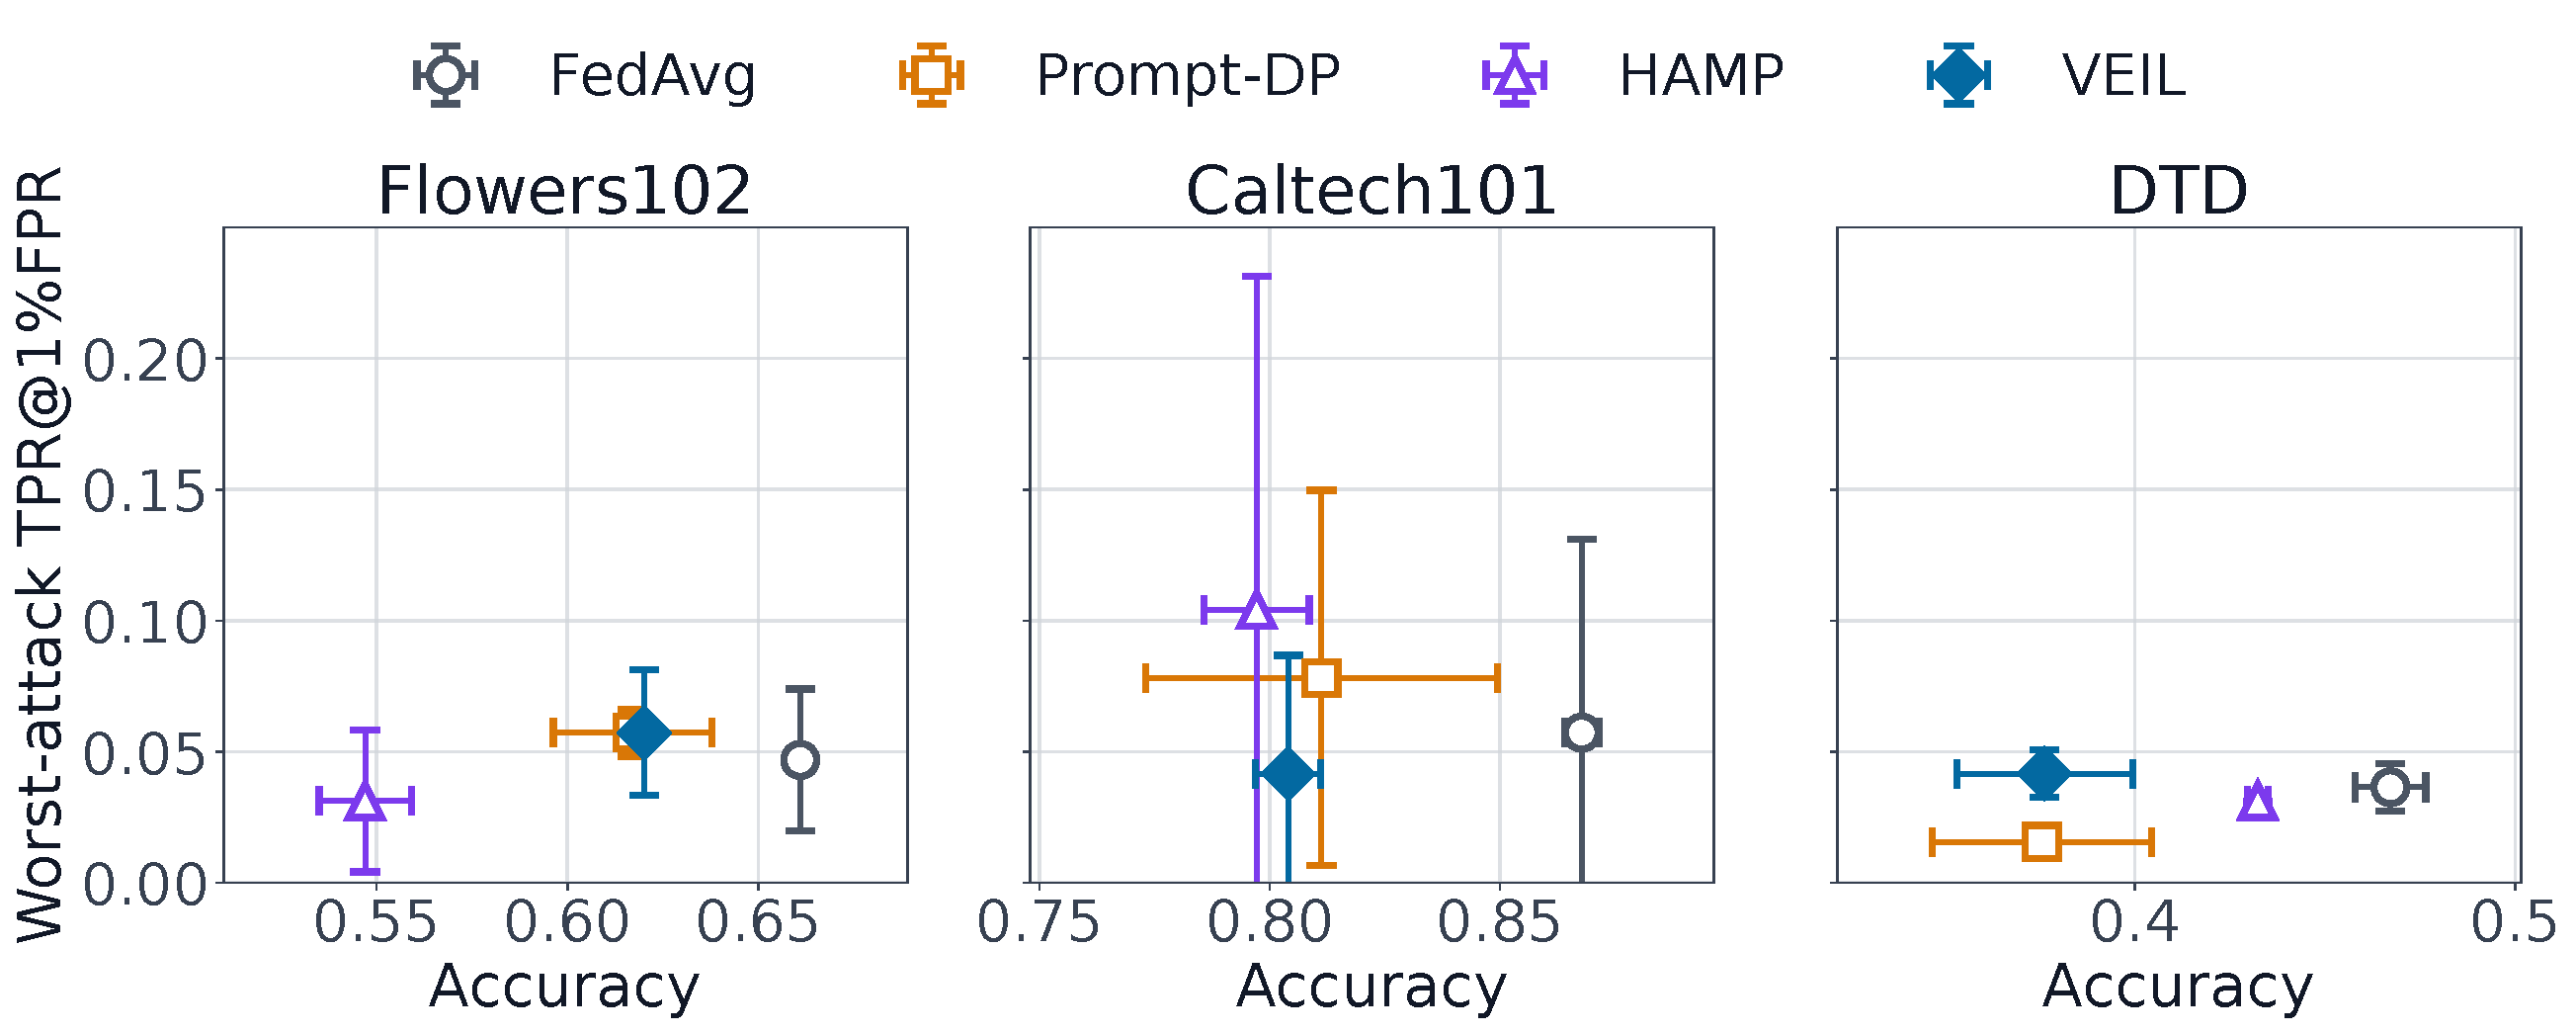
\includegraphics[width=0.96\textwidth]{figures/fedavg_privacy_utility.pdf}
\caption{FedAvg privacy--utility comparison across Flowers102, Caltech101, and
DTD.  Points report seed means; horizontal and vertical bars show one sample
standard deviation.  The vertical scale is shared; horizontal ranges are
panel-specific and explicitly labeled.  Lower worst-attack \tpr{} and higher
accuracy are better.}
\label{fig:fedavg}
\end{figure*}

\begin{table*}[t]
\centering
\begin{tabular}{llccc}
\toprule
Dataset & Defense & Accuracy $\uparrow$ & Worst \tpr{} $\downarrow$ & Mean \tpr{} $\downarrow$\\
\midrule
Flowers102 & No defense & 0.6609 $\pm$ 0.0030 & 0.0469 $\pm$ 0.0271 & 0.0191 $\pm$ 0.0066\\
Flowers102 & Prompt-DP & 0.6170 $\pm$ 0.0207 & 0.0573 $\pm$ 0.0090 & 0.0191 $\pm$ 0.0080\\
Flowers102 & HAMP & 0.5471 $\pm$ 0.0120 & 0.0313 $\pm$ 0.0271 & 0.0122 $\pm$ 0.0143\\
Flowers102 & \method{} & 0.6201 $\pm$ 0.0013 & 0.0573 $\pm$ 0.0239 & 0.0113 $\pm$ 0.0066\\
Caltech101 & No defense & 0.8677 $\pm$ 0.0037 & 0.0573 $\pm$ 0.0738 & 0.0148 $\pm$ 0.0157\\
Caltech101 & Prompt-DP & 0.8112 $\pm$ 0.0382 & 0.0781 $\pm$ 0.0716 & 0.0278 $\pm$ 0.0330\\
Caltech101 & HAMP & 0.7971 $\pm$ 0.0115 & 0.1042 $\pm$ 0.1273 & 0.0321 $\pm$ 0.0296\\
Caltech101 & \method{} & 0.8040 $\pm$ 0.0070 & 0.0417 $\pm$ 0.0451 & 0.0130 $\pm$ 0.0158\\
DTD & No defense & 0.4672 $\pm$ 0.0093 & 0.0365 $\pm$ 0.0090 & 0.0130 $\pm$ 0.0045\\
DTD & Prompt-DP & 0.3755 $\pm$ 0.0289 & 0.0156 $\pm$ 0.0000 & 0.0043 $\pm$ 0.0015\\
DTD & HAMP & 0.4323 $\pm$ 0.0027 & 0.0312 $\pm$ 0.0000 & 0.0130 $\pm$ 0.0026\\
DTD & \method{} & 0.3762 $\pm$ 0.0231 & 0.0417 $\pm$ 0.0090 & 0.0191 $\pm$ 0.0030\\
\bottomrule
\end{tabular}
\caption{FedAvg defenses under identical data, optimization, participation, and
audit settings.  Values are mean $\pm$ sample standard deviation over seeds
42--44.}
\label{tab:fedavg}
\end{table*}

On Flowers102, \method{} retains the highest accuracy among the three defenses
(0.6201), narrowly above Prompt-DP and substantially above HAMP.  HAMP attains
the lowest worst-attack TPR, whereas \method{} attains the lowest six-attack
mean.  The undefended model nevertheless has both higher accuracy and a lower
measured worst-attack TPR than \method{} on this dataset.  This counterexample
underscores that a finite empirical audit is neither monotone in defense
strength nor a proxy for formal privacy: VEIL suppresses leakage on average but
does not dominate every attack realization.  We therefore interpret the full
per-attack, cross-dataset profile rather than declaring a universal winner.

On Caltech101, \method{} gives the strongest privacy summary among the three
defenses: worst-attack and mean \tpr{} are 0.0417 and 0.0130, compared with
0.0781/0.0278 for Prompt-DP and 0.1042/0.0321 for HAMP.  Its 0.8040 accuracy is
6.38 percentage points below the undefended model, but is comparable to the two
defenses.  DTD reverses the conclusion.  Prompt-DP reaches the lowest worst and
mean \tpr{} (0.0156/0.0043), whereas \method{} reaches 0.0417/0.0191 and loses
9.10 accuracy points relative to no defense.  Averaged equally over datasets,
\method{} has accuracy 0.6001, worst-attack \tpr{} 0.0469, and mean \tpr{}
0.0145.  The latter is 15.3\% and 24.2\% relatively below Prompt-DP and HAMP,
but the DTD failure rules out a dataset-independent superiority claim.

\subsection{Attack Profiles under DP-FPL and FedASK}

The second study holds the audit fixed and changes the federated training
mechanism.  Figure~\ref{fig:private} shows that a single aggregate privacy score
can hide attack-specific failures; we therefore retain all six columns in
Table~\ref{tab:private}.

\begin{figure*}[t]
\centering
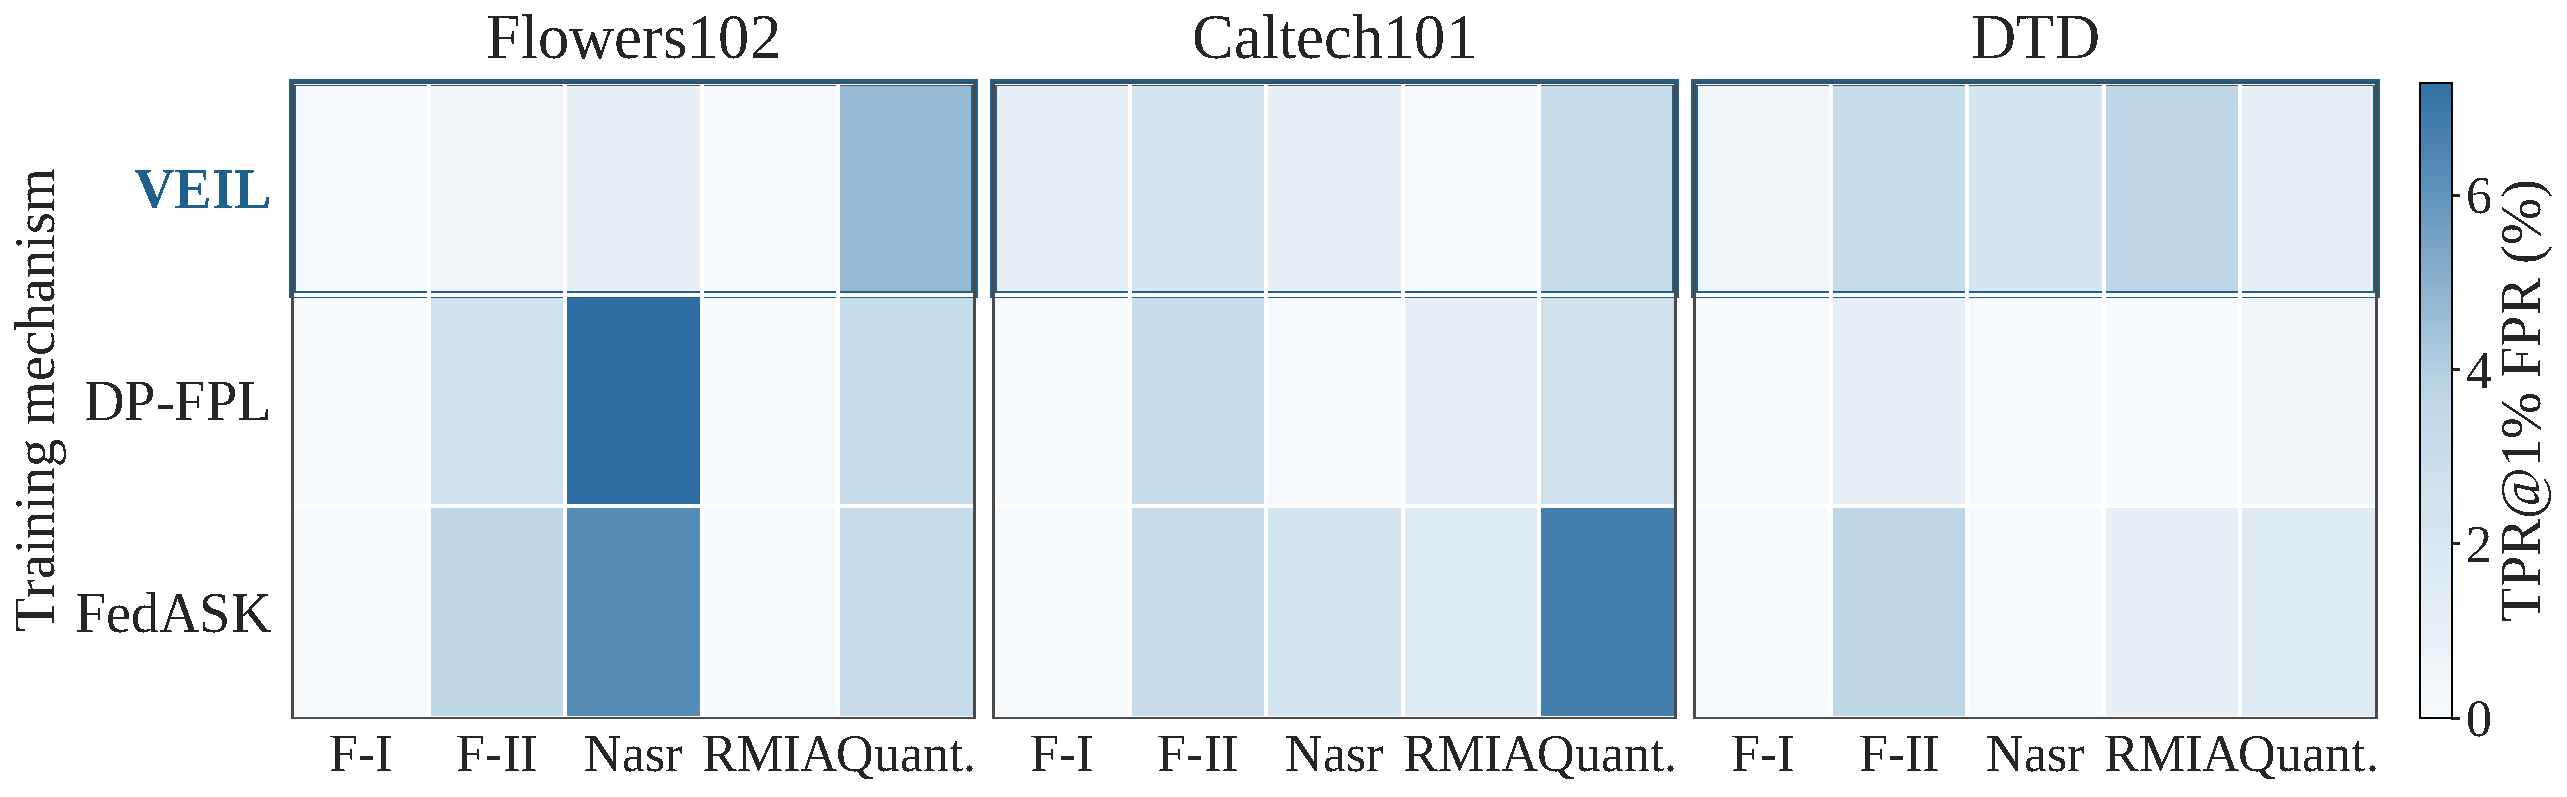
\includegraphics[width=0.96\textwidth]{figures/private_methods_attack_profile.pdf}
\caption{Per-attack \tpr{} for DP-FPL and FedASK, averaged over seeds 42--44.
Panels share a common zero-based scale; lower bars indicate less empirical
membership leakage.}
\label{fig:private}
\end{figure*}

\begin{table*}[t]
\centering
\begin{tabular}{llcccccc}
\toprule
Dataset & Method & Loss & Cosine & Joint & Nasr & RMIA & Quantile\\
\midrule
Flowers102 & DP-FPL & 0.0000 & 0.0260 & 0.0260 & 0.0729 & 0.0000 & 0.0312\\
Flowers102 & FedASK & 0.0000 & 0.0365 & 0.0208 & 0.0625 & 0.0000 & 0.0312\\
Caltech101 & DP-FPL & 0.0000 & 0.0312 & 0.0104 & 0.0000 & 0.0104 & 0.0260\\
Caltech101 & FedASK & 0.0000 & 0.0312 & 0.0208 & 0.0208 & 0.0156 & 0.0677\\
DTD & DP-FPL & 0.0000 & 0.0104 & 0.0208 & 0.0000 & 0.0000 & 0.0052\\
DTD & FedASK & 0.0000 & 0.0365 & 0.0417 & 0.0000 & 0.0104 & 0.0156\\
\bottomrule
\end{tabular}
\caption{Attack-specific \tpr{} under private federated training mechanisms.
Values are seed means.  ``Loss'', ``Cosine'', and ``Joint'' denote the three
FedMIA variants.}
\label{tab:private}
\end{table*}

Nasr is the strongest mean attack on Flowers102 for both DP-FPL (0.0729) and
FedASK (0.0625).  The ordering changes with the dataset: on Caltech101,
FedMIA-Cosine is largest for DP-FPL (0.0312), while Quantile MIA is largest for
FedASK (0.0677); on DTD, FedMIA-Joint is largest for both mechanisms
(0.0208/0.0417).  DP-FPL also has higher mean accuracy than FedASK on all three
datasets---0.5552 versus 0.5270, 0.7428 versus 0.6063, and 0.3557 versus
0.3330.  Both mechanisms show substantial seed variability; for example,
FedASK's Caltech101 accuracy has sample standard deviation 0.2308.  Changes in
the strongest attacker motivate retaining the full attack profile.

\begin{table}[t]
\centering
\begin{tabular}{llcc}
\toprule
Method & Scope & $\epsilon$ upper bound & $\delta$\\
\midrule
Prompt-DP & prompt update & 46.51--81.51 & $10^{-5}$\\
DP-FPL & local & 122.62 & $10^{-5}$\\
DP-FPL & global & 511.51 & $10^{-5}$\\
FedASK & local & 61.51 & $10^{-5}$\\
\bottomrule
\end{tabular}
\caption{Conservative Gaussian-RDP accounting over all nine runs per mechanism.
No client or example subsampling amplification is claimed.  Prompt-DP varies
with the maximum client step count; the other reported bounds are constant.
These large upper bounds do not establish strong privacy at the selected noise
settings.}
\label{tab:accounting}
\end{table}

\subsection{Cross-Dataset Attack Surface}

Figure~\ref{fig:heatmap} provides a compact attack-by-method view.  The shared
color scale is anchored at zero and the numeric labels prevent color-only
interpretation.  This view is diagnostic: the worst-attack aggregation remains
the decision metric because a defense should not be selected by averaging away
one effective attacker.

\begin{figure*}[t]
\centering
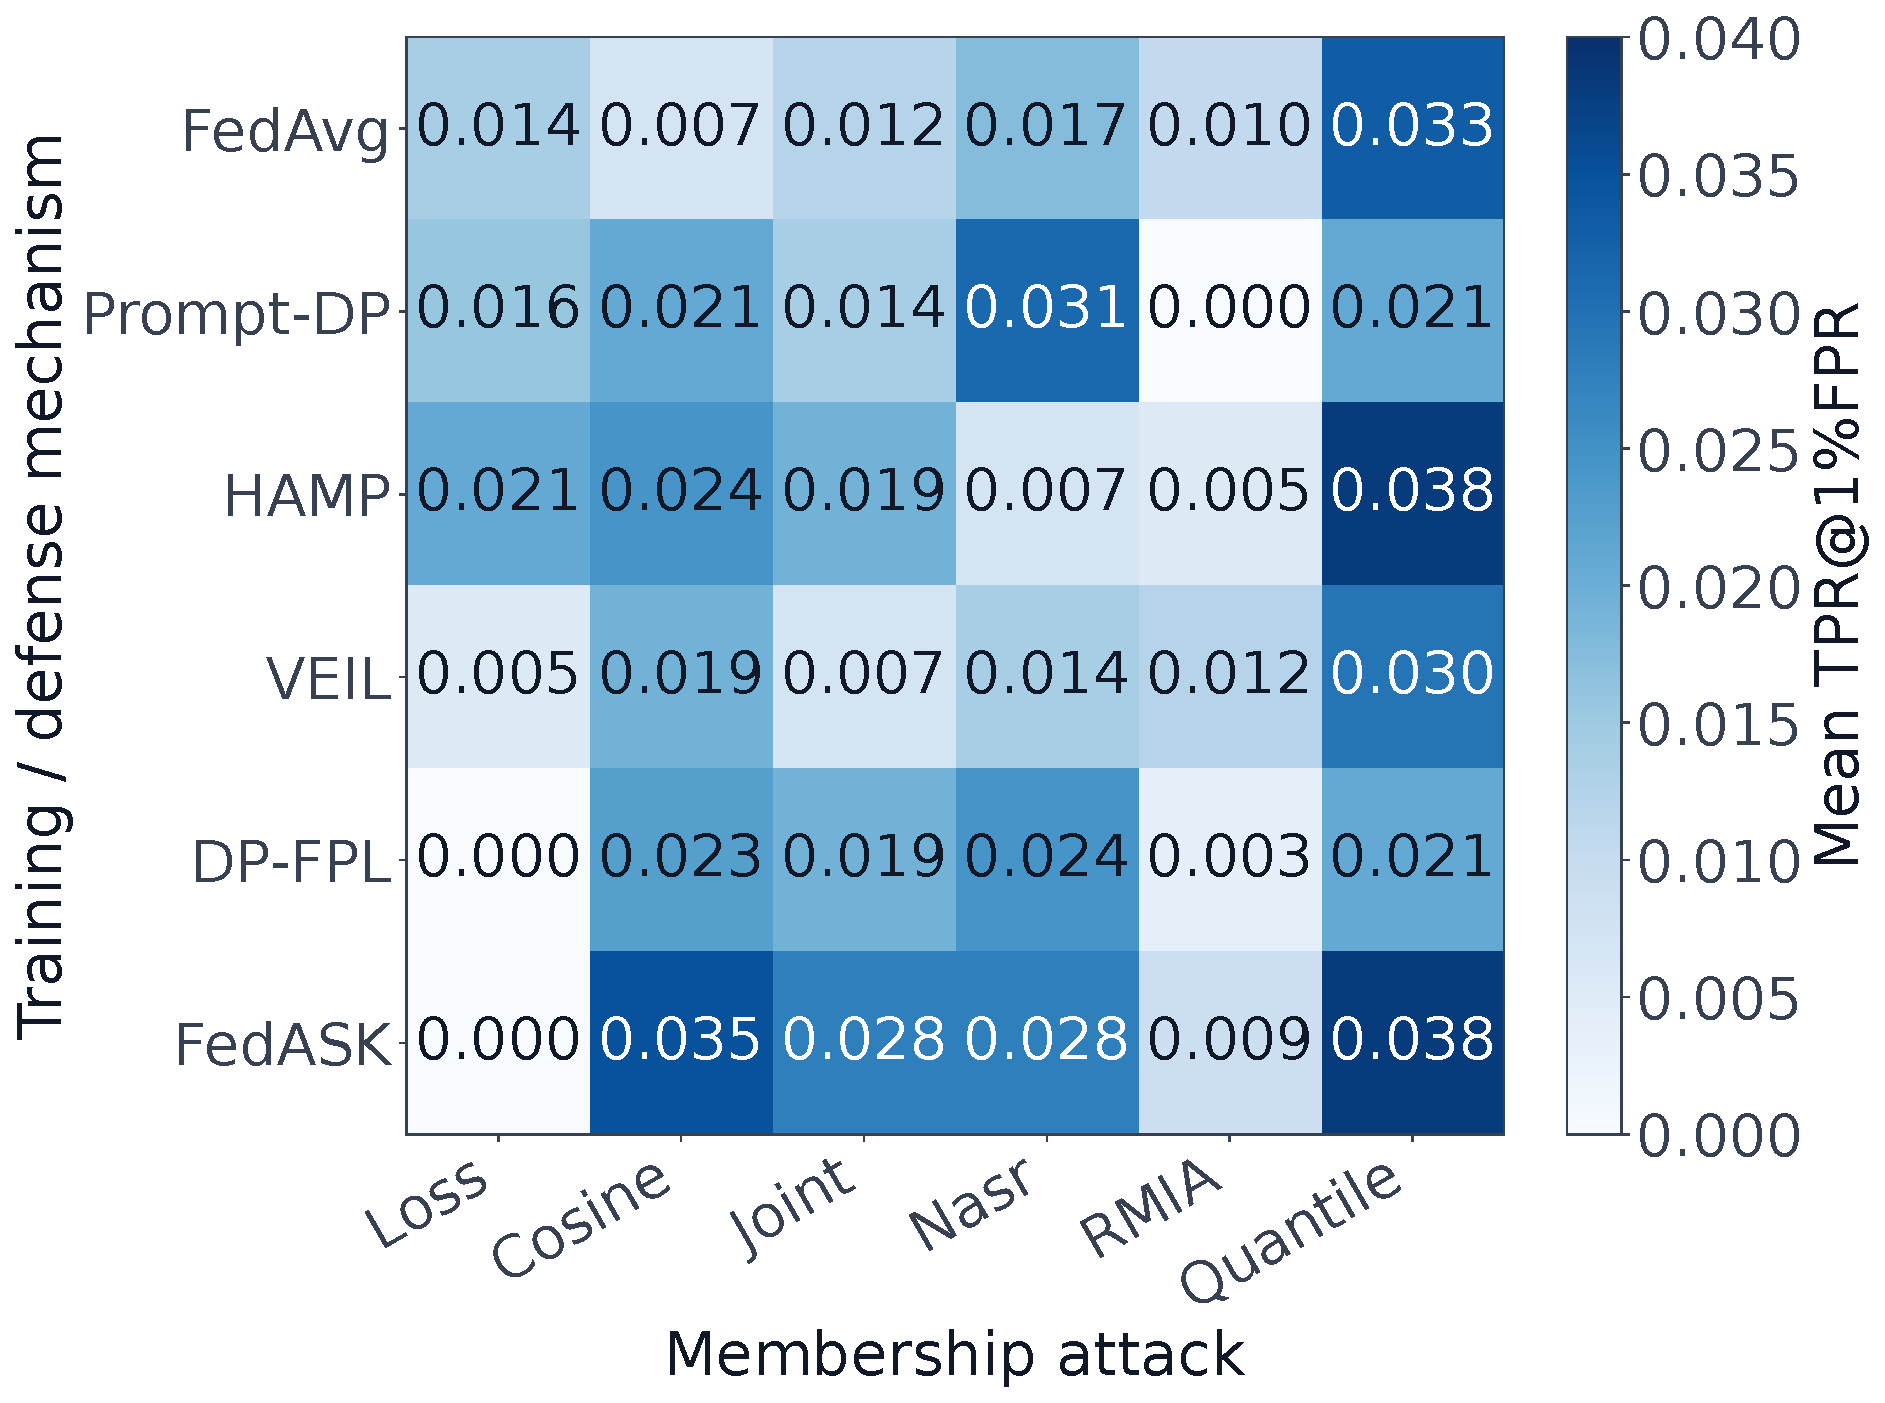
\includegraphics[width=0.96\textwidth]{figures/attack_defense_heatmap.pdf}
\caption{Cross-dataset mean \tpr{} by attack and training/defense mechanism.
Every cell is the unweighted mean over the three datasets and three seeds.}
\label{fig:heatmap}
\end{figure*}

\subsection{Component Analysis}

The Flowers102 seed-42 component study varies one design choice at a time.  Full
\method{} obtains accuracy 0.6216, worst-attack \tpr{} 0.0312, and mean \tpr{}
0.0052.  Removing upload smoothing raises accuracy to 0.6515 but doubles the
worst statistic to 0.0625 and increases the attack mean to 0.0182, making
smoothing the clearest privacy--utility lever in this diagnostic.  Replacing the
class anchor by an individual feature doubles mean \tpr{} to 0.0104; removing
echoes raises it to 0.0078.  Removing the prototype branch, or removing output
tempering, leaves both privacy summaries unchanged at this resolution.  The
latter is expected for rank-based ROC metrics when positive temperature scaling
does not change score order.  Adding noise to the prototype also leaves the
privacy summaries unchanged while reducing accuracy to 0.6154.  Because this is
a single-seed diagnostic, these equalities should not be generalized beyond the
measured operating point.

\begin{figure}[t]
\centering
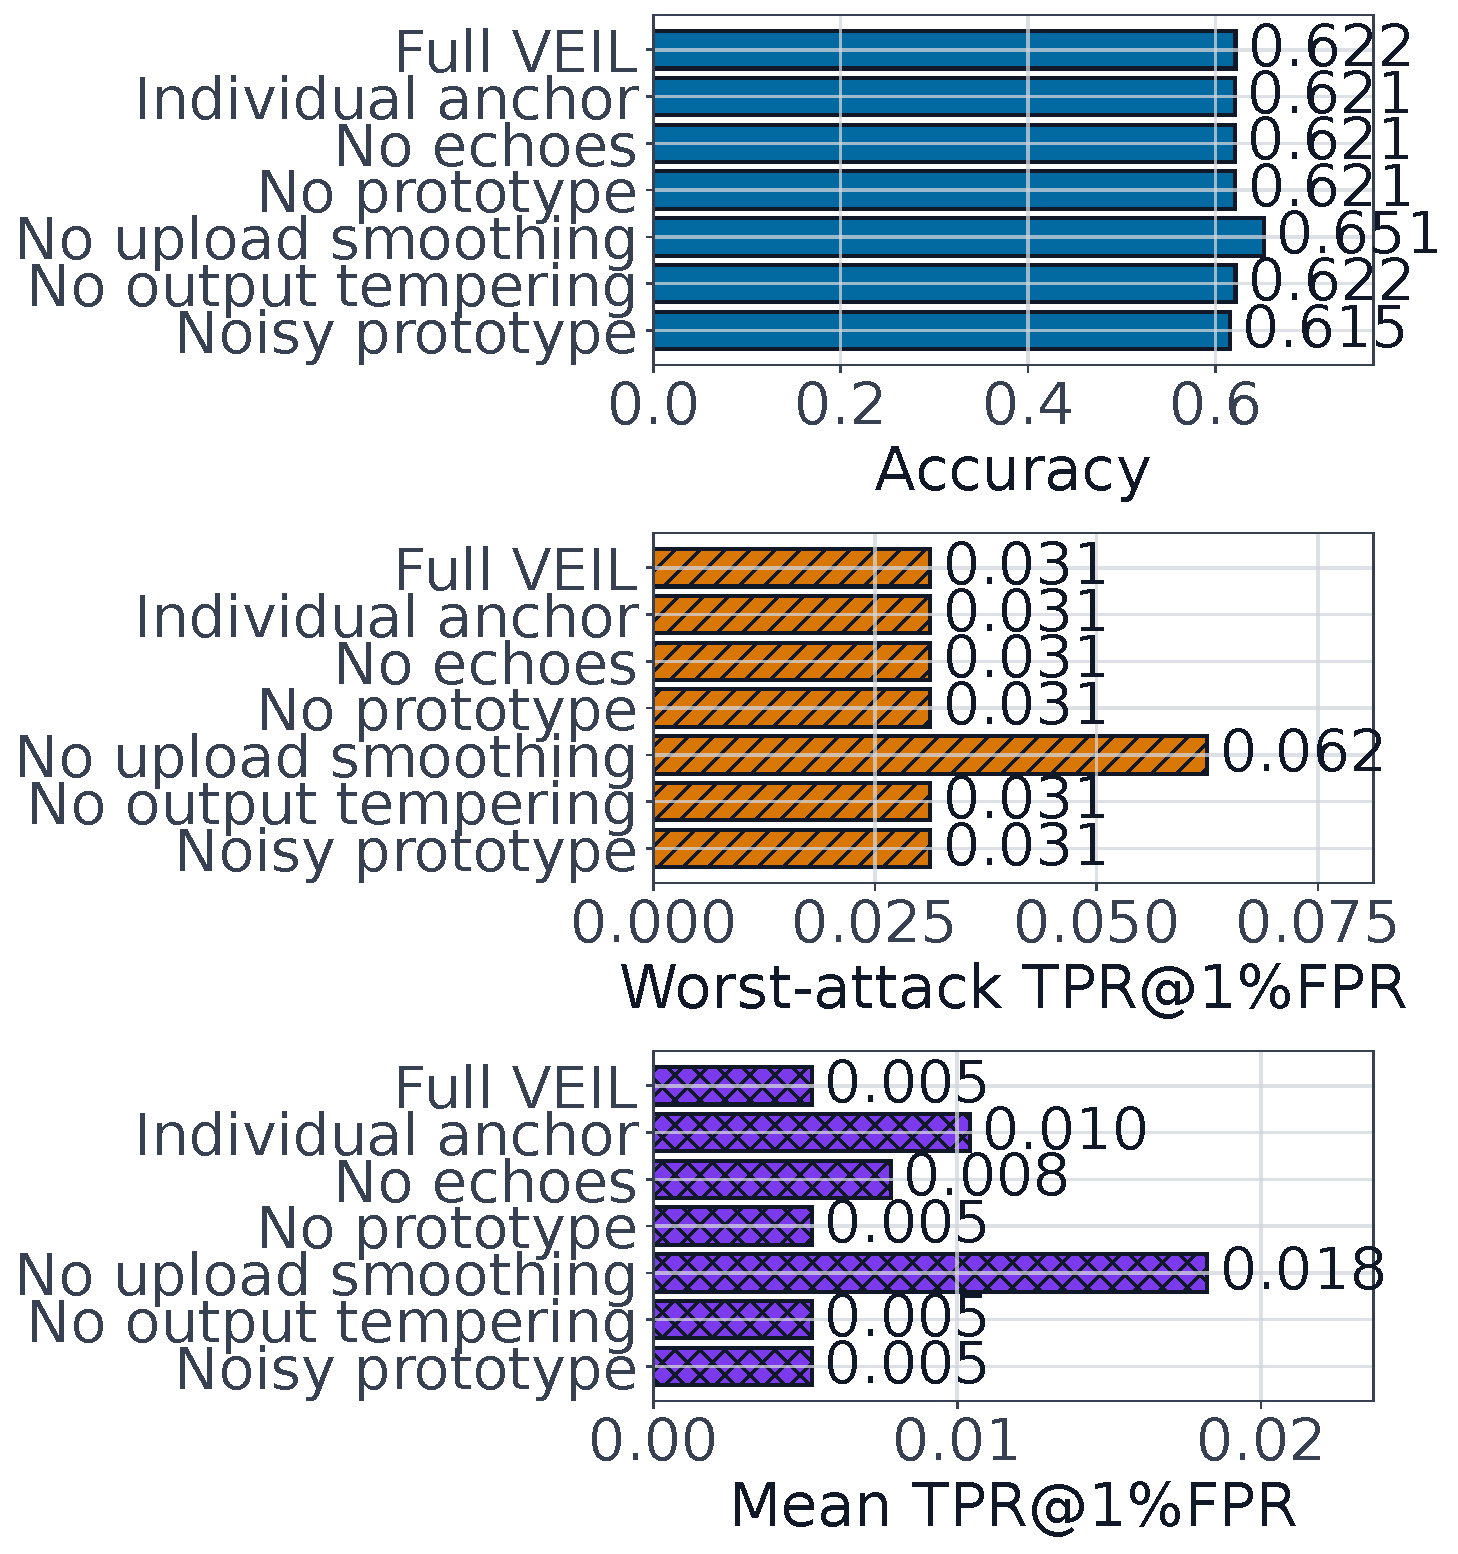
\includegraphics[width=0.96\columnwidth]{figures/veil_ablation.pdf}
\caption{\method{} component ablation on Flowers102 seed 42.  Accuracy,
worst-attack \tpr{}, and six-attack mean \tpr{} are shown on separate aligned
panels rather than a dual axis; this diagnostic is not presented as a
repeated-seed estimate.}
\label{fig:ablation}
\end{figure}

\section{Limitations}

\method{} provides empirical resistance to the audited attacks, not formal
differential privacy.  A low measured \tpr{} can reflect finite candidate
resolution---including the zero-false-positive threshold described above---and
no finite attack suite proves the absence of leakage.  Our
experiments freeze one CLIP architecture, use full client participation, and
consider three image datasets; partial participation, larger backbones, other
modalities, and adaptive attackers remain open.  Prototype replacement can also
under-represent rare within-class modes, while Gaussian upload smoothing may be
inappropriate when downstream users require deterministic updates.  The DTD
result is a concrete transfer failure: Flowers102-tuned VEIL reduces accuracy
without improving either privacy summary, so cross-dataset retuning or adaptive
scaling remains necessary.

\section{Ethical Statement}

The intended benefit is reducing disclosure of whether a person's example was
used during collaborative adaptation.  The same mechanism could conceal data
provenance or complicate accountability if deployed without audit logs.  We
therefore recommend reporting both empirical attack results and any formal
privacy accounting, preserving model/data documentation, and avoiding claims
that federated learning alone guarantees privacy.

\section{Conclusion}

We presented \method{}, a local geometric-echo defense for federated CLIP
prompt learning.  By replacing individual image anchors with class prototypes,
sampling local covariance-shaped echoes, and smoothing only the uploaded prompt
delta, then tempering released logits, \method{} targets representation-,
protocol-, and final-query-side membership
signals without transmitting additional client statistics.  A label-matched,
RNG-isolated audit across multiple attacks and datasets provides a stricter basis
for comparison than accuracy or AUC alone.  VEIL gives the lowest cross-dataset
mean attack TPR among the evaluated FedAvg defenses, yet its DTD failure shows
that the trade-off is data dependent.  Distributional surrogate training is
therefore a practical empirical complement to DP-FPL, FedASK, and output-centered
defenses, while formal guarantees remain the domain of explicitly accounted
mechanisms.

\bibliography{veil}

\input{veil_reproducibility.tex}

\end{document}
